\section{Experiments}
\label{sec:experiments}
We evaluate predicted latency, search cost, and recovered schedules. Studies include prefill/decode and fixed-hardware mapping. For example, the full-input DeepSeek case
adds autoregressive decode and phase-specific controls. TPU-v3 provides a
publicly documented reference baseline consistent with prior
work~\citep{jouppi2021ten,zhang_fast}. All speedups below are analytical and modeled results.

\subsection{Experimental Setup}
\label{sec:exp_intro}
The suite comprises EfficientNet-B1--B7, Llama-1 13B/65B,
Llama-3 70B, and DeepSeek-V3~\citep{tan2019efficientnet,llama3modelcard,deepseekv3report} and Stable Diffusion~1.5 UNet.
The campaign compares static pinning, fixed-tile temporal
placement, and joint tiling under the same cost convention. These are restricted
controls of CHEETAH, not separate proposed systems. Small programs use
HiGHS~\citep{huangfu2018parallel}; operator-based native working programs use OCS.
The new BF16 suite recovery enumerates a finite common-chip menu and minimizes
independent implementation or stage choices within each candidate. These
recovered executions are evaluated separately from continuous LP certificates.
The full-input experiment binds actual checkpoint routes and preserves every
logical invocation (Appendix~\ref{app:native_provenance}).

The new checkpoint-bound comparisons use the same numerical contract on both
arms: BF16 matrix operands and activations, FP32 accumulation and the pinned
implementation's sensitive operations, with TF32 and reduced-precision
accumulation disabled. Checkpoint conversion and data movement are charged.
Historical prefill results retain their original numerical and workload
contracts; we do not combine their speedups with the new BF16 results.

\paragraph{Physical Design Validation.} Since modeling simulations ultimately present a gap with real world physical performance, we validate all results through a five-level audit process: (i) Roofline Auditor, (ii) Campaign Validator, (iii) Causal Ledger, (iv) solver diagnostics, and (v) six pre-RTL gates. Each CHEETAH design must pass all five audit tiers before it is deemed feasible and reported. 

The roofline check rejects costs below compute or memory service floors.
Table~\ref{tab:mfg_gates} lists the architectural screening thresholds. These are modeling checks, not fabricated-chip timing or packaging sign-off.
RTL and synthesis evidence is in Appendix~\ref{sec:rtl_validation}.

\begin{table}[t]
\centering\small
\caption{Six architectural feasibility gates.}
\label{tab:mfg_gates}
\begin{tabularx}{\linewidth}{@{}lXr@{}}
\toprule
Gate & Check & Threshold \\
\midrule
Pin count & HBM3-class signal pins at $0.8$ GB/s/pin & $\le4{,}096$ \\
Reticle area & Linear area model at 7 nm & $\le600$ mm$^2$ \\
Logic depth & MAC-tree combinational depth & $\le35$ levels \\
NoC routing & $n_{\rm PEs}\,n_{\rm banks}$ & $\le5\times10^6$ cells \\
Power density & Dynamic power / die area & $\le2.0$ W/mm$^2$ \\
SRAM macros & 64 KiB banks, aspect ratio $1{:}4$--$4{:}1$ & $\le4{,}096$ banks \\
\bottomrule
\end{tabularx}
\end{table}

\subsection{Reported Efficiency Quantities}
\label{sec:reported_quantities}
Three quantities carry the efficiency claims below, and each is read off the
scheduled execution rather than assumed. Let $T$ be the duration of the
interval being reported, $C_{\mathrm{peak}}$ the peak arithmetic throughput of
the recovered chip, $b_r$ the peak bandwidth of resource $r$, and
$P_{\mathrm{peak}}$ its modeled peak power.
\begin{equation}
\mathrm{MFU}=\frac{F_{\mathrm{useful}}}{C_{\mathrm{peak}}T},
\qquad
\mathrm{MBU}_r=\frac{B_{r,\mathrm{read}}+B_{r,\mathrm{write}}}{b_rT},
\qquad
\mathrm{Perf}/\mathrm{TDP}=\frac{Q/T}{P_{\mathrm{peak}}}.
\label{eq:reported_quantities}
\end{equation}

\paragraph{Model FLOP utilization.}
$\mathrm{MFU}$ is the fraction of the chip's arithmetic capability that the
schedule converts into useful work, where $F_{\mathrm{useful}}$ counts only the
arithmetic the model requires. It is distinct from the work the arrays actually
issue: padding, masked edge tiles and replicated operands are charged to the
machine but are not useful, so $F^{\mathrm{useful}}\le F^{\mathrm{issued}}$
always. Within a fixed-chip branch the per-event service rows enforce
$\sum_i F^{\mathrm{issued}}_{i,e}x_{i,e}\le C_{\mathrm{peak}}\Delta t_e$, which
sums every concurrent implementation sharing the arrays in event $e$; because
the installed rate is a branch constant there, summing over the event intervals
guarantees an aggregate $\mathrm{MFU}\le 1$ by construction rather than by
inspection. This guarantee is a property of the fixed-chip rows and is not
inherited by the variable-hardware relaxation, where the corresponding product
is bilinear and its McCormick envelope is necessary but not exact
(\cref{app:physical_rooflines}); the installed-rate condition is therefore
re-checked exactly at execution admission.

\paragraph{Model bandwidth utilization.}
$\mathrm{MBU}_r$ is the same ratio for a memory resource, and it is computed
from the \emph{complete} scheduled traffic: operand rereads, KV transfers
between timesteps, and spill and restore movement all count, since each
occupies the interface whether or not it advances the model's arithmetic.
Because the resources have different peak rates and different consequences for
a schedule, HBM, the host link and on-chip SRAM are reported separately rather
than aggregated into a single figure.

\paragraph{Performance per TDP.}
$\mathrm{Perf}/\mathrm{TDP}$ divides delivered throughput, $Q$ units of work
per unit time, by modeled peak power. Three conditions govern its use as a
comparison. The process, the power scope and the unit of work must match
between the designs compared; a ratio across differing scopes is not a ratio of
efficiencies. Average measured power is not a substitute for modeled peak TDP,
and we do not interchange them. And because the objective minimizes latency
rather than this ratio, a performance/power tradeoff is obtained by solving
across power budgets and comparing recovered designs: for a fixed amount of
work the ratio factors as
$(\mathrm{Perf}/\mathrm{TDP})_{\mathrm{design}}/(\mathrm{Perf}/\mathrm{TDP})_{\mathrm{baseline}}
=(T_{\mathrm{baseline}}/T_{\mathrm{design}})\cdot(\mathrm{TDP}_{\mathrm{baseline}}/\mathrm{TDP}_{\mathrm{design}})$,
so a latency objective does not by itself maximize it.

All three are reported over the prefill interval, the decode interval, and the
whole task separately, because a quantity averaged across phases conceals the
regime change between them. Values recovered from a fractional relaxation are
reported as bounds, not as admitted physical designs; only points that survive
integral recovery and replay are reported as designs.

\subsection{Workload Results and Fixed-Hardware Controls}
\label{sec:prog}\label{sec:fixed_hw}
The original campaign reports an average $22.07\times$ predicted
speedup over its modeled TPU-v3 baseline, reaching $40.1\times$ on Llama-3 70B.
These are prefill-oriented results under that campaign's workload and traffic
conventions. Appendix~\ref{app:blueprints} shows the concrete hardware blueprints;
Appendix~\ref{app:original_results} has the original plots and restricted
controls. 

\paragraph{Uniform BF16 extension.}
The following archived comparisons use the earlier host-backed reference and
physical-cost coefficients. They are not yet verified comparisons against
FAST's modeled TPU-v3 baseline. The BF16 power and interface correction in
Appendix~\ref{app:native_feasibility_repair} requires new chip recovery;
the original numerical records are retained here with that scope.
Table~\ref{tab:uniform_bf16_cnn} applies the DeepSeek comparison convention to
fresh EfficientNet-B1--B7 and UNet captures. Each classifier result covers one complete classifier
forward at its original resolution, cold checkpoint conversion/import and final
output writeback. The reference uses the same frozen matrix mapper and scaling,
900 GB/s DRAM, 32 GB/s host service, 2,048 vector lanes and 8,192 GB/s local
service as the reported DeepSeek comparison. These latter service rates are
analytical assumptions. The software control retains the reference matrix
implementations while keeping intermediate tensors in DRAM and vector
temporaries in registers.

The custom search selects a common chip and independent per-invocation tiles
from a finite recovery family. Convolution may materialize patches or read them
directly; direct reads pay 24 scalar address/mask cycles per issued input
element. The execution serializes transfers and kernels, retains all observed
classifier allocations in DRAM, and charges FP32-checkpoint-to-BF16 conversion.
Rational replay checks every original invocation, dependency, allocation,
transfer and selected service count. This is analytical recovery, not a
full-master optimality certificate or a measurement of the custom kernels.

\begin{table}[t]
\centering\small
\caption{Archived BF16 vision predictions, including preparation and writeback.
All latencies are ms. SW holds the modeled TPU-v3 resources fixed.}
\label{tab:uniform_bf16_cnn}
\begin{tabular}{@{}lrrrr@{}}
\toprule
Workload & Reference & Reference + SW & Custom & Speedup \\
\midrule
EfficientNet-B1 & 13.657 & 3.557 & 0.826 & $16.53\times$ \\
EfficientNet-B2 & 17.124 & 4.372 & 1.011 & $16.94\times$ \\
EfficientNet-B3 & 28.752 & 7.276 & 1.576 & $18.25\times$ \\
EfficientNet-B4 & 59.880 & 15.673 & 3.128 & $19.14\times$ \\
EfficientNet-B5 & 117.697 & 29.791 & 5.946 & $19.79\times$ \\
EfficientNet-B6 & 200.960 & 53.037 & 9.859 & $20.38\times$ \\
EfficientNet-B7 & 354.137 & 97.591 & 16.909 & $20.94\times$ \\
SD1.5 UNet (50 calls) & 109,439.059 & 55,112.649 & 2,712.737 & $40.34\times$ \\
\bottomrule
\end{tabular}
\end{table}

B1--B4 select 512 $16\times16$ arrays and 114 MiB SRAM; B5--B7 select 896
arrays and 185.875 MiB SRAM. Both designs have 16,384 vector lanes,
2,608 GB/s DRAM and 32,768 GB/s local service. Their host interfaces supply
512 and 256 GB/s respectively. Area/power proxies are 411.64 mm$^2$/295.55 W
and 523.44 mm$^2$/298.47 W under the earlier coefficient set. These old power
values do not establish compliance with the repaired 300-W BF16 model.
This comparison includes the explicit interface provisioning difference.
The seven fixed-resource software controls improve predicted latency by
$3.63$--$3.95\times$; full co-design gives $16.53$--$20.94\times$.
Classifiers and denoising UNets have no autoregressive prefill/decode split.

\paragraph{Same-chip feature controls.}
Table~\ref{tab:uniform_bf16_cnn_controls} removes one implementation freedom
at a time while retaining the recovered chip, all original operations and
their order, DRAM residence, cold preparation and output writeback. Direct
affine convolution reads avoid materializing patches, after paying their
address generation and masked reads. Per-invocation tiling chooses different
matrix tiles for different operations. Its control uses the best single
tile from the same five-tile menu for the whole network, while preserving
independent convolution dataflow choices. All resulting schedules pass rational
replay. These effects interact and are not additive; the controls optimize
their declared serial implementation menus, not every feature-disabled schedule.

\begin{table}[t]
\centering\small
\caption{Latency relative to the full BF16 design on the same chip.
Larger values show the cost of removing a feature.}
\label{tab:uniform_bf16_cnn_controls}
\begin{tabular}{@{}lrr@{}}
\toprule
Workload & Materialized patches only & Best single matrix tile \\
\midrule
EfficientNet-B1 & $2.00\times$ & $1.040\times$ \\
EfficientNet-B2 & $2.07\times$ & $1.049\times$ \\
EfficientNet-B3 & $2.15\times$ & $1.064\times$ \\
EfficientNet-B4 & $2.29\times$ & $1.065\times$ \\
EfficientNet-B5 & $2.38\times$ & $1.090\times$ \\
EfficientNet-B6 & $2.44\times$ & $1.096\times$ \\
EfficientNet-B7 & $2.48\times$ & $1.103\times$ \\
\bottomrule
\end{tabular}
\end{table}

\paragraph{Denoising UNet.}
The UNet result covers all 50 captured denoising calls; conditioning, the
scheduler and image decoding remain outside that declared boundary. Its chip
has 1,024 arrays, 209.75 MiB SRAM and a 128-GB/s host interface, with the same
vector, DRAM and local service rates. A paid 128-KiB GELU table is checked over
every finite BF16 input and all original tensor layouts; positional tables are
recomputed from their captured constant programs. Preparation contributes
32.508 ms and denoising with boundary transfers 2,680.229 ms. The result is an
analytical UNet design, not a complete text-to-image timing measurement.
On this same chip, restricting GELU to one banked lookup-table copy increases
latency from 2,712.737 to 7,304.729 ms ($2.693\times$); the full design chooses
the number of table replicas per operation and pays their bank capacity and
reload traffic. Materializing every convolution patch increases latency to
2,987.345 ms ($1.101\times$). In contrast, the best common matrix tile gives
2,713.233 ms, only $1.00018\times$ slower. Thus adaptive tiling contributes
little for this UNet, whereas lookup replication is consequential. Each control
retains the original 50 calls, numerical table, chip and boundary transfers;
their effects are not additive.

\paragraph{Common comparison across the suite.}
Table~\ref{tab:uniform_suite_overview} preserves the archived designs under
the BF16/FP32 arithmetic and modeled reference convention used for DeepSeek.
Each ratio compares the same complete declared task on the two chips;
task sizes differ across models and are specified below. Cold preparation
is included. The historical host-backed reference is not yet verified against
FAST's modeled TPU-v3 baseline, and these chips require re-screening under the
consistent BF16 physical-cost contract (Appendix~\ref{app:native_feasibility_repair}).
The hardware and software controls following the table identify
which changes contribute, without adding interacting speedup ratios.

\begin{table}[t]
\centering\small
\caption{Archived ratios over the earlier host-backed TPU-v3-resource reference; baseline and BF16 physical-cost reconciliation remain open. Phase ratios do not add. Dashes denote inapplicable phases.}
\label{tab:uniform_suite_overview}
\begin{tabular}{@{}lrrr@{}}
\toprule
Workload & Overall & Prefill & Decode \\
\midrule
EfficientNet-B1 & $16.53\times$ & -- & -- \\
EfficientNet-B2 & $16.94\times$ & -- & -- \\
EfficientNet-B3 & $18.25\times$ & -- & -- \\
EfficientNet-B4 & $19.14\times$ & -- & -- \\
EfficientNet-B5 & $19.79\times$ & -- & -- \\
EfficientNet-B6 & $20.38\times$ & -- & -- \\
EfficientNet-B7 & $20.94\times$ & -- & -- \\
SD1.5 UNet (50 calls) & $40.34\times$ & -- & -- \\
Llama-1 13B & $122.59\times$ & $48.00\times$ & $148.94\times$ \\
Llama-1 65B & $68.92\times$ & $25.36\times$ & $80.76\times$ \\
Llama-3 70B & $91.78\times$ & $47.14\times$ & $105.93\times$ \\
DeepSeek-V3 & $31.71\times$ & $19.85\times$ & $37.93\times$ \\
\bottomrule
\end{tabular}
\end{table}

\paragraph{Full-inference Llama designs.}
The same BF16/FP32 arithmetic and reference service rates apply to 32
independent requests per model, each producing 512 greedy output tokens.
Llama-1 retains its original 1,536-token prompt; Llama-3 uses 4,096 tokens.
Prefill emits the first output, followed by 511 decode forwards per request.
Cold checkpoint conversion/import and final backing are charged in every arm.
These are modeled extensions of the paper reference convention, not measured
TPU serving latencies. The reference remains the original host-backed
singleton schedule; the software arm holds all reference resources fixed.

Recovery selects a common chip and compatible linear batches. Between linear
stages, each member executes its original dependent operations, keeping
attention temporaries private. Gather/scatter, KV copies and all original
token dependencies are retained. Whole immutable parameters may remain in
DRAM across stages and timesteps after their first paid import. Their complete
extents are conservatively reserved in addition to the original KV/activation
peak. A bounded residency MILP selects these leases. The fixed-resource
software arm also batches linears and shares weights within each stage,
using memory-feasible complete-request cohorts and the same matrix mapper.
These finite recovery searches provide analytical executions; the separate
DeepSeek LP certificate is not transferred to them.

\begin{table}[t]
\centering\scriptsize
\caption{Uniform full-inference predictions in seconds for all 32 requests. Preparation is included in totals. SW keeps TPU-v3 resources fixed.}
\label{tab:uniform_llama_phases}
\begin{tabular}{@{}llrrrr@{}}
\toprule
Model & Phase & Reference & Reference + SW & Custom & Speedup \\
\midrule
Llama-1 13B & Prefill & 980.380 & 720.526 & 20.425 & $48.00\times$ \\
 & Decode & 17,668.410 & 1,317.840 & 118.631 & $148.94\times$ \\
 & Total & 18,663.574 & 2,053.150 & 152.245 & $122.59\times$ \\
\addlinespace
Llama-1 65B & Prefill & 4,407.777 & pending & 173.827 & $25.36\times$ \\
 & Decode & 82,145.424 & pending & 1,017.176 & $80.76\times$ \\
 & Total & 86,627.355 & pending & 1,256.908 & $68.92\times$ \\
\addlinespace
Llama-3 70B & Prefill & 15,076.868 & 10,905.168 & 319.824 & $47.14\times$ \\
 & Decode & 106,905.123 & 7,982.193 & 1,009.241 & $105.93\times$ \\
 & Total & 121,981.992 & 18,887.361 & 1,329.065 & $91.78\times$ \\
\addlinespace
\bottomrule
\end{tabular}
\end{table}

Llama-1 13B selects 512 $16\times16$ arrays, 16,384 vector lanes, 114 MiB SRAM and a 512-GB/s host interface (411.64 mm$^2$/295.55 W proxies). Its 43,350,816 logical operations complete in 1 cohort(s) of 32 requests. It retains 275 parameters occupying 13.416 GiB; the conservative DRAM bound is 63.998 GiB within 64 GiB. Prefill/decode account for 5.19\%/94.81\% of predicted time saved; preparation is separate. Fixed-resource software improves the reference by $9.09\times$; the custom design is a further $13.49\times$ faster.

Llama-1 65B selects 128 $16\times16$ arrays, 12,288 vector lanes, 74.375 MiB SRAM and a 1,024-GB/s host interface (326.38 mm$^2$/298.15 W proxies). Its 114,898,464 logical operations complete in 4 cohort(s) of 8 requests. It retains 335 parameters occupying 23.045 GiB; the conservative DRAM bound is 64.000 GiB within 64 GiB. Prefill/decode account for 4.96\%/95.03\% of predicted time saved; preparation is separate.

Llama-3 70B selects 512 $16\times16$ arrays, 16,384 vector lanes, 114 MiB SRAM and a 512-GB/s host interface (411.64 mm$^2$/295.55 W proxies). Its 133,248,544 logical operations complete in 1 cohort(s) of 32 requests. It retains 373 parameters occupying 11.241 GiB; the conservative DRAM bound is 63.997 GiB within 64 GiB. Prefill/decode account for 12.23\%/87.77\% of predicted time saved; preparation is separate. Fixed-resource software improves the reference by $6.46\times$; the custom design is a further $14.21\times$ faster.

All custom designs retain 64-GiB DRAM and use the same paid memory-interface
and local-service model as DeepSeek. These comparisons include differences
in installed interface bandwidth. Local and A100 replays check service and
logical memory; physical fragmentation and silicon timing are not measured.

\begin{table}[t]
\centering\scriptsize
\caption{Matched custom-chip controls. Extra predicted time in seconds relative to each retained design; effects are not additive.}
\label{tab:uniform_llama_controls}
\begin{tabular}{@{}llrrr@{}}
\toprule
Model & Control & Prefill extra & Decode extra & Latency ratio \\
\midrule
Llama-1 13B & No linear batching & 0.000 & 222.329 & $2.460\times$ \\
 & Singletons, no weight leases & 2.298 & 1,417.469 & $10.326\times$ \\
 & KV spill/restore & 0.115 & 137.112 & $1.901\times$ \\
 & No cross-step weight residency & 0.000 & 20.976 & $1.138\times$ \\
\addlinespace
Llama-1 65B & No linear batching & 0.000 & 1,324.921 & $2.054\times$ \\
 & Singletons, no weight leases & 6.969 & 4,909.761 & $4.912\times$ \\
 & KV spill/restore & 0.242 & 287.970 & $1.229\times$ \\
 & No cross-step weight residency & 0.139 & 94.616 & $1.075\times$ \\
\addlinespace
Llama-3 70B & No linear batching & 0.000 & 1,175.788 & $1.885\times$ \\
 & Singletons, no weight leases & 12.443 & 7,551.977 & $6.692\times$ \\
 & KV spill/restore & 0.124 & 134.051 & $1.101\times$ \\
 & No cross-step weight residency & 0.000 & 17.593 & $1.013\times$ \\
\addlinespace
\bottomrule
\end{tabular}
\end{table}




In the historical controls, Table~\ref{tab:fixed_hw} holds each chip
fixed and compares the joint schedule against streaming every tensor. The
compact NPU has $32{,}768$ INT8 MACs at 1 GHz, 64 GB/s bandwidth, and 16 MiB
on-chip storage; TPU-v3 uses the original 900 GB/s, 32 MiB model. The larger
NPU gains reflect its tighter memory bandwidth. No hardware-area normalization
is needed within a same-chip pair.

\begin{table}[t]
\centering\small
\caption{Historical fixed-chip speedup, under the original numerical contracts.}
\label{tab:fixed_hw}
\begin{tabular}{@{}lrr@{}}
\toprule
Workload & TPU-v3 & Compact NPU \\
\midrule
Llama-1 13B & $2.14\times$ & $31.4\times$ \\
Llama-3 70B & $2.51\times$ & $7.66\times$ \\
DeepSeek-V3 & $2.22\times$ & $7.8\times$ \\
SD1.5 UNet & $1.50\times$ & $5.89\times$ \\
\midrule
Geometric mean & $2.06\times$ & $10.3\times$ \\
\bottomrule
\end{tabular}
\end{table}

\subsection{Search Cost and LLM Guidance}
\label{sec:breakdown}
Cached implementation coefficients remove repeated mapper calls from the inner
search. In the original 50-trial comparison, joint tiling reduces Llama-70B
search time from $58.42$ to $1.17$ hours and DeepSeek-V3 from $69.39$ to $2.17$
hours relative to the fixed-tile temporal pipeline. These are search times,
not inference speedups. The LLM-guided campaign reduces mean invalid trials
from $24.5\%$ to $5.9\%$ while reaching the same best observed Perf/TDP score
as its full-space Vizier control. This tests proposal efficiency, not proof of
an optimal architecture or causal validity of every dual suggestion.


% ---- plots restored from the long version, original placement ----

\begin{figure}[ht!]
    \centering
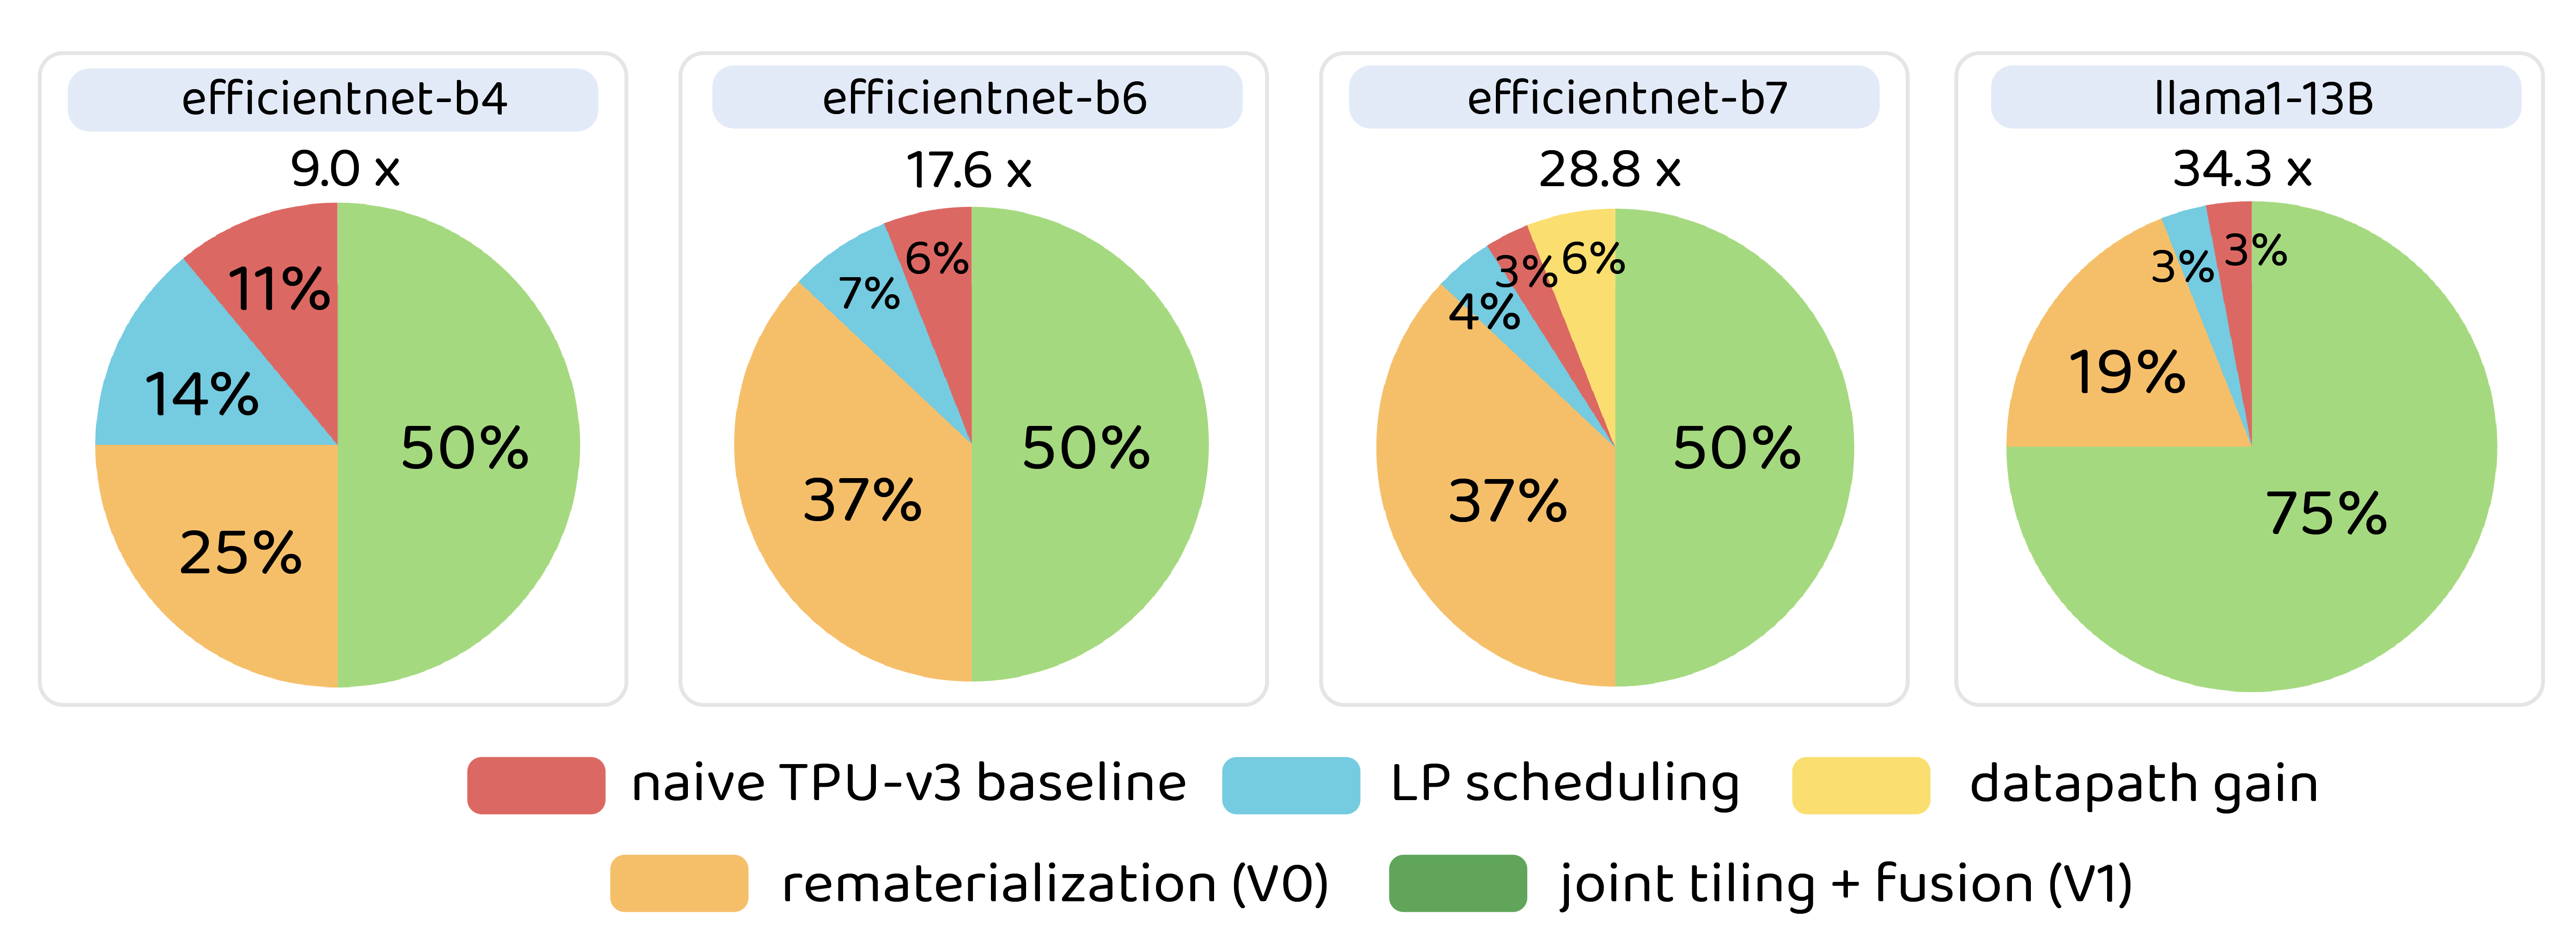
\includegraphics[width=0.85\linewidth]{fig3/speedup_decomposition_final_v4.png}
\caption{Retained historical prefill attribution under the original campaign's numerical and traffic conventions. The artwork's V1 label denotes joint tiling and fusion. New uniform BF16 phase and feature controls are reported separately in Tables~\ref{tab:uniform_llama_phases}, \ref{tab:uniform_llama_controls}, and \ref{tab:uniform_bf16_cnn_controls}.}\label{fig:accel_decompose}
\end{figure}

\begin{figure}[ht!] 
    \centering
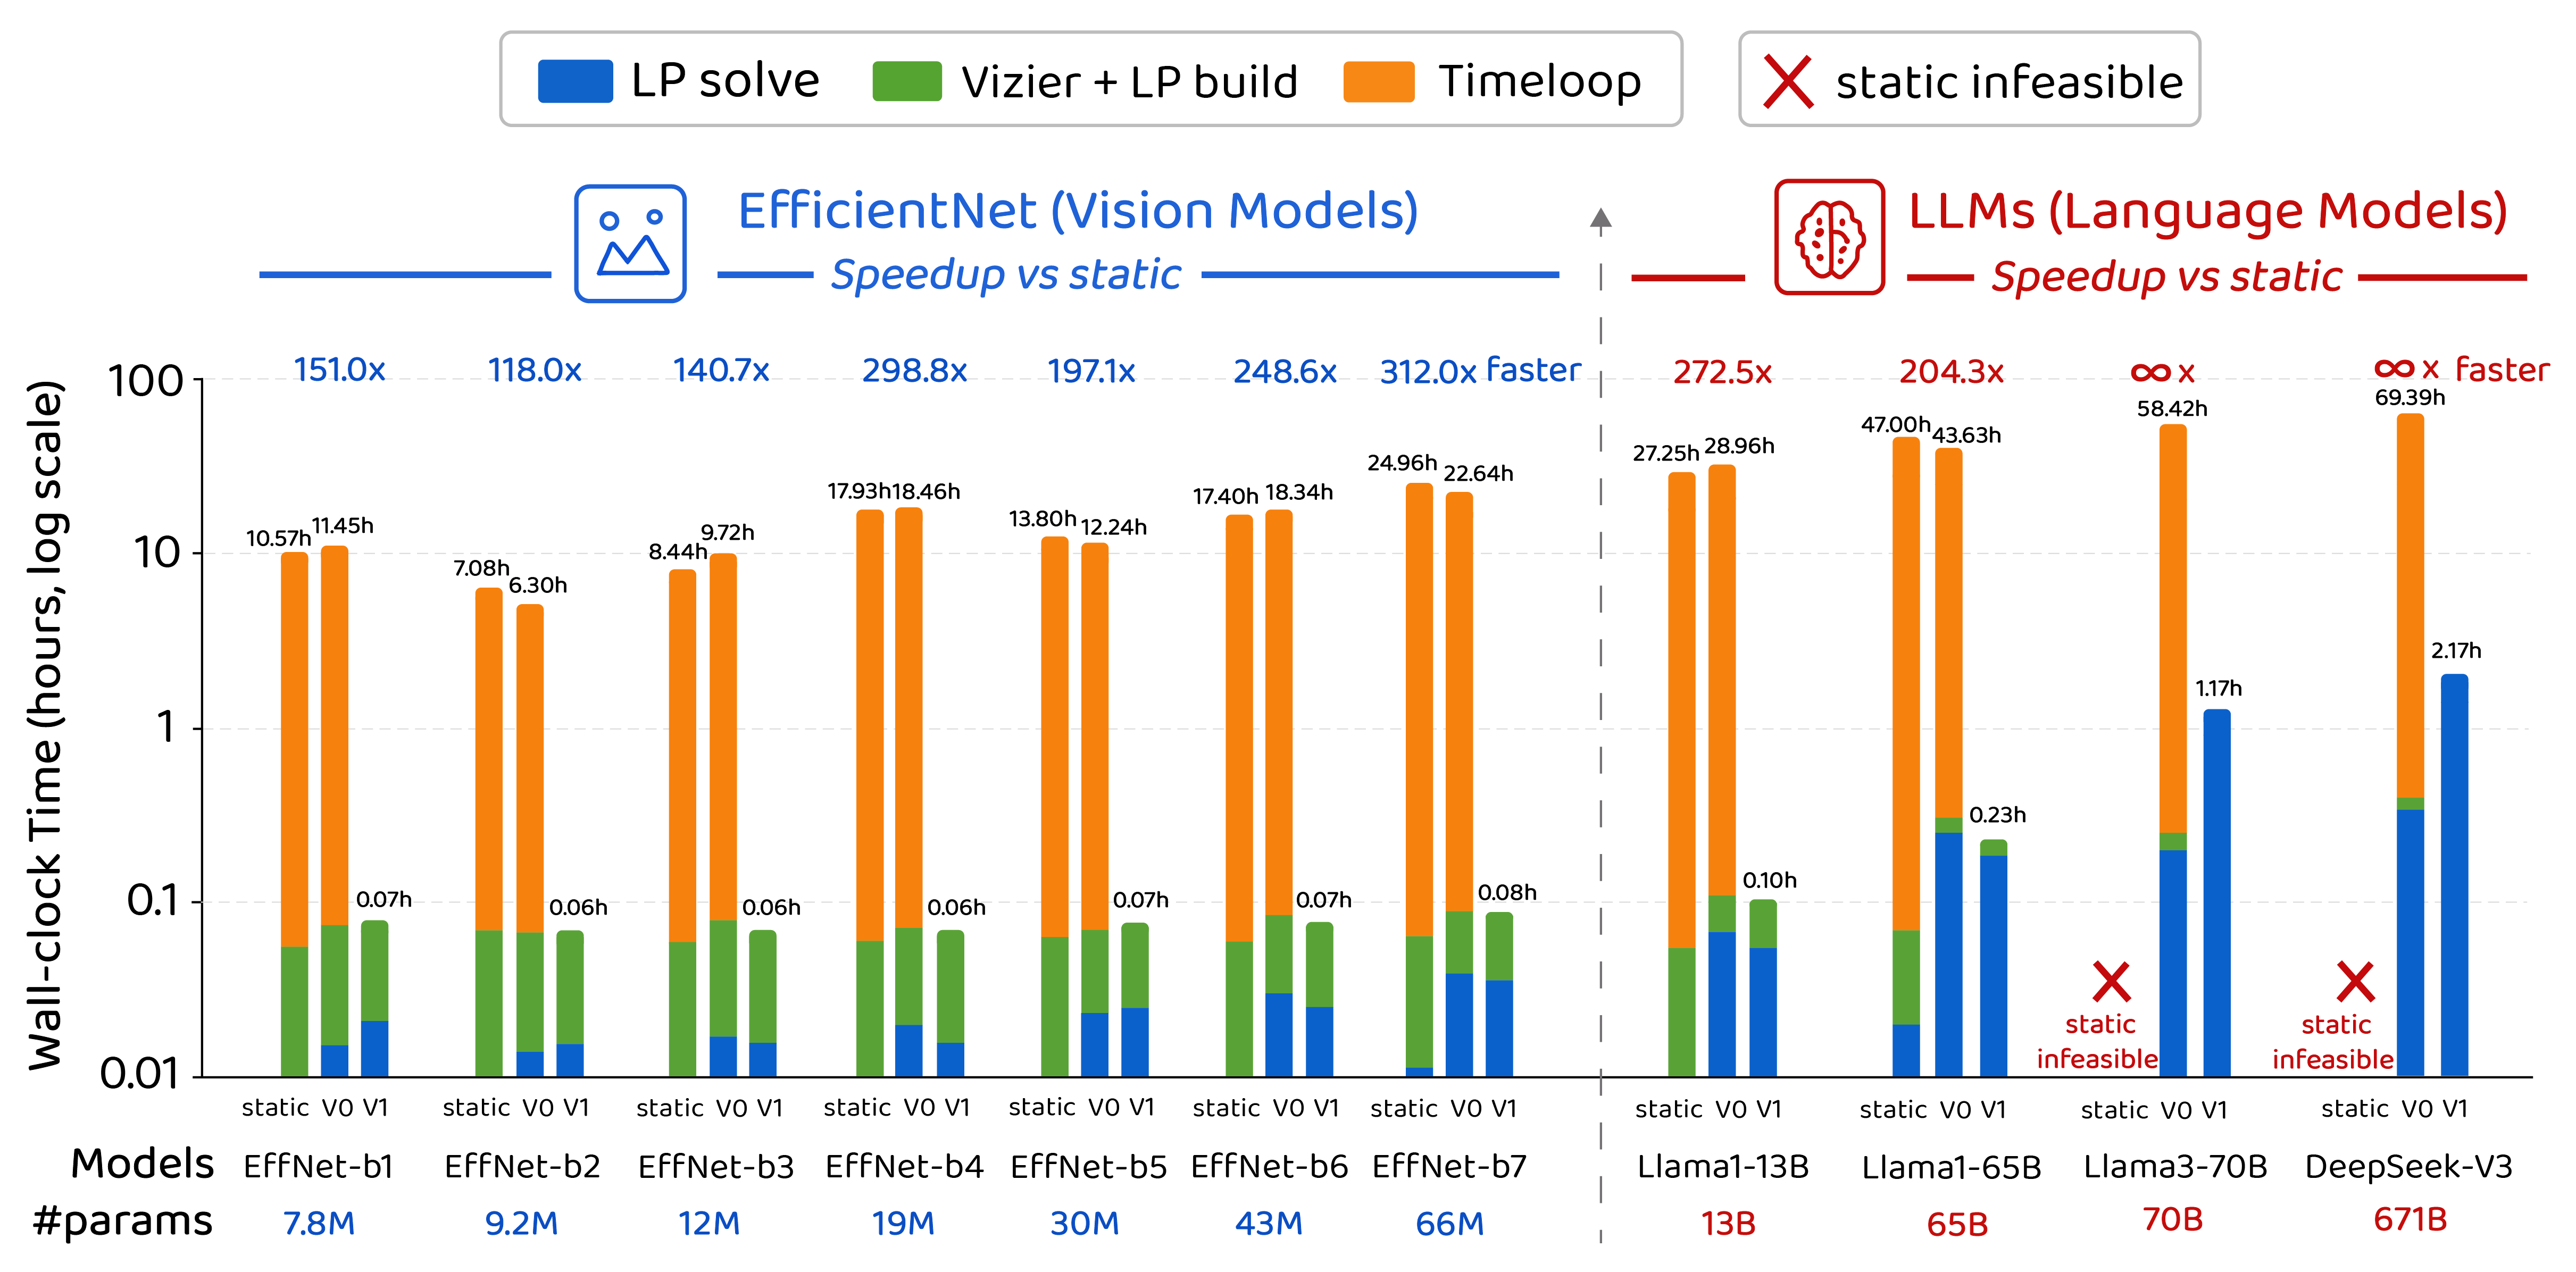
\includegraphics[width=1.0\linewidth]{fig3/wallclock_new_v6.png}
\caption{Wall-clock time decomposition and performance acceleration across formulations: CHEETAH-V1's internalized tiling eliminates the Timeloop bottleneck, achieving up to 100--300$\times$ faster search than the classical static method. Upper bars show wall-clock hours (log scale); annotations show speedup vs.\ static.}
\label{fig:wallclock}
\end{figure}

\begin{figure}[h]
\centering
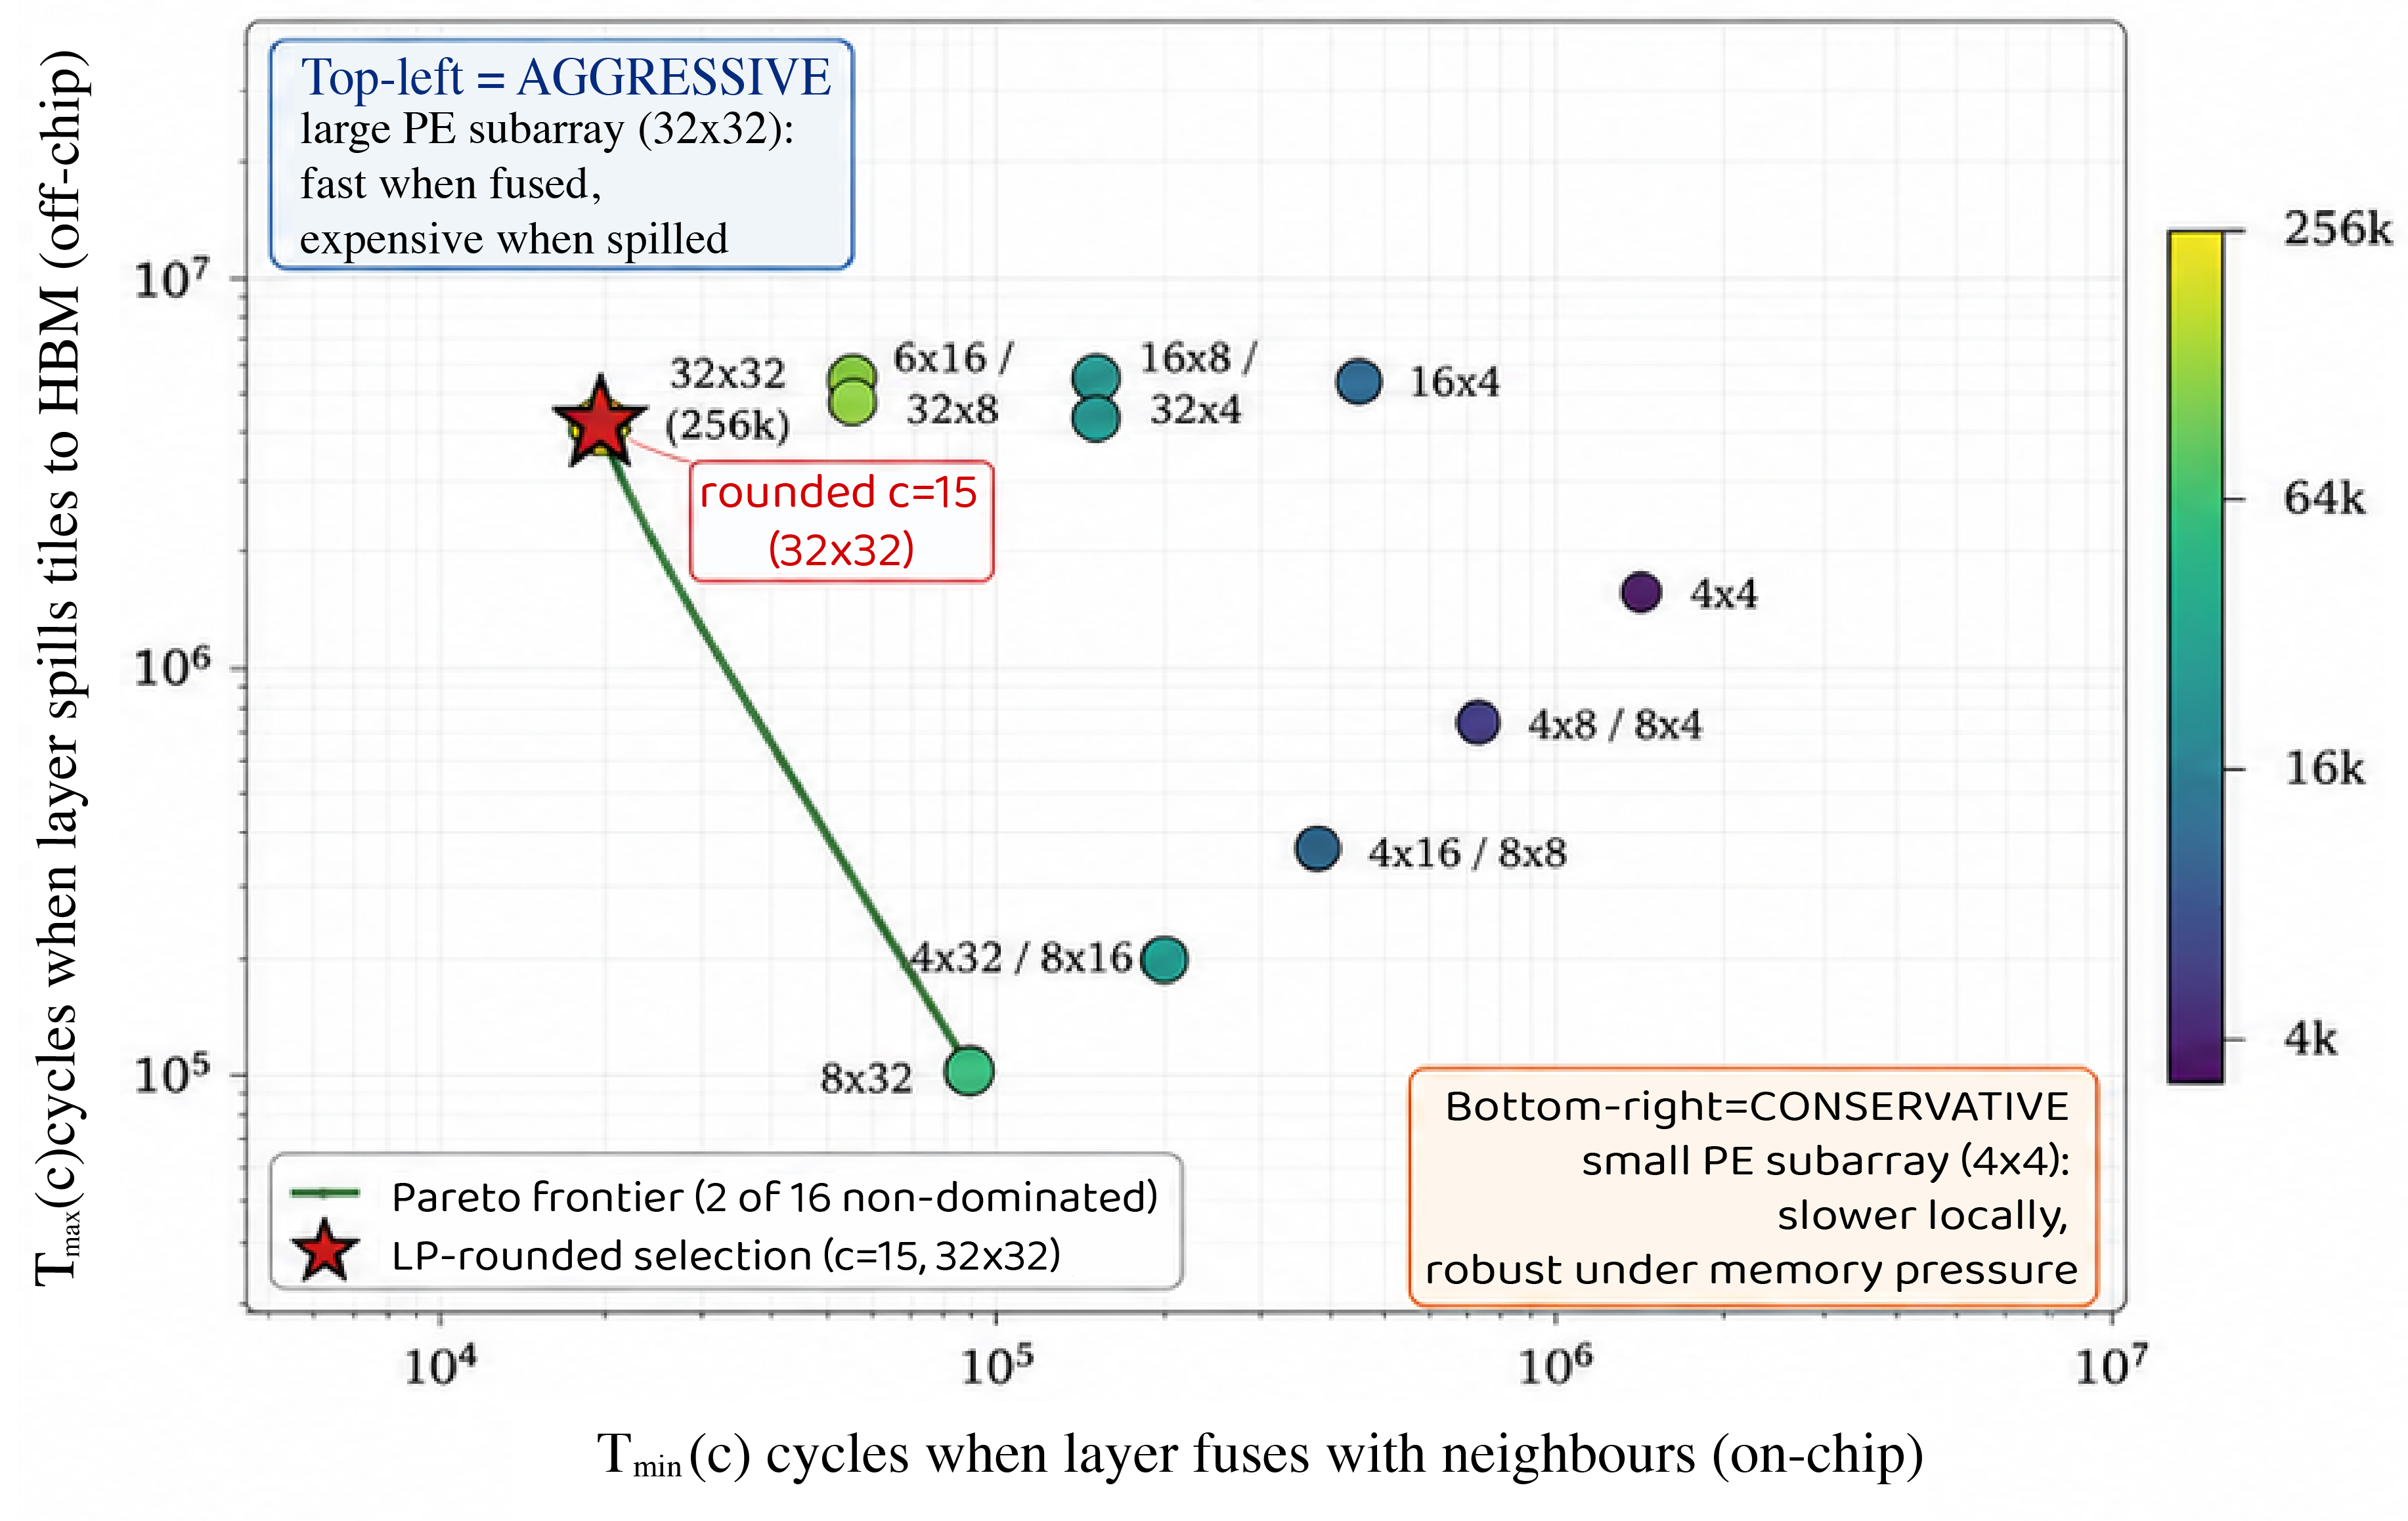
\includegraphics[width=0.48\textwidth]{figs4/pareto_front.png}
\hfill
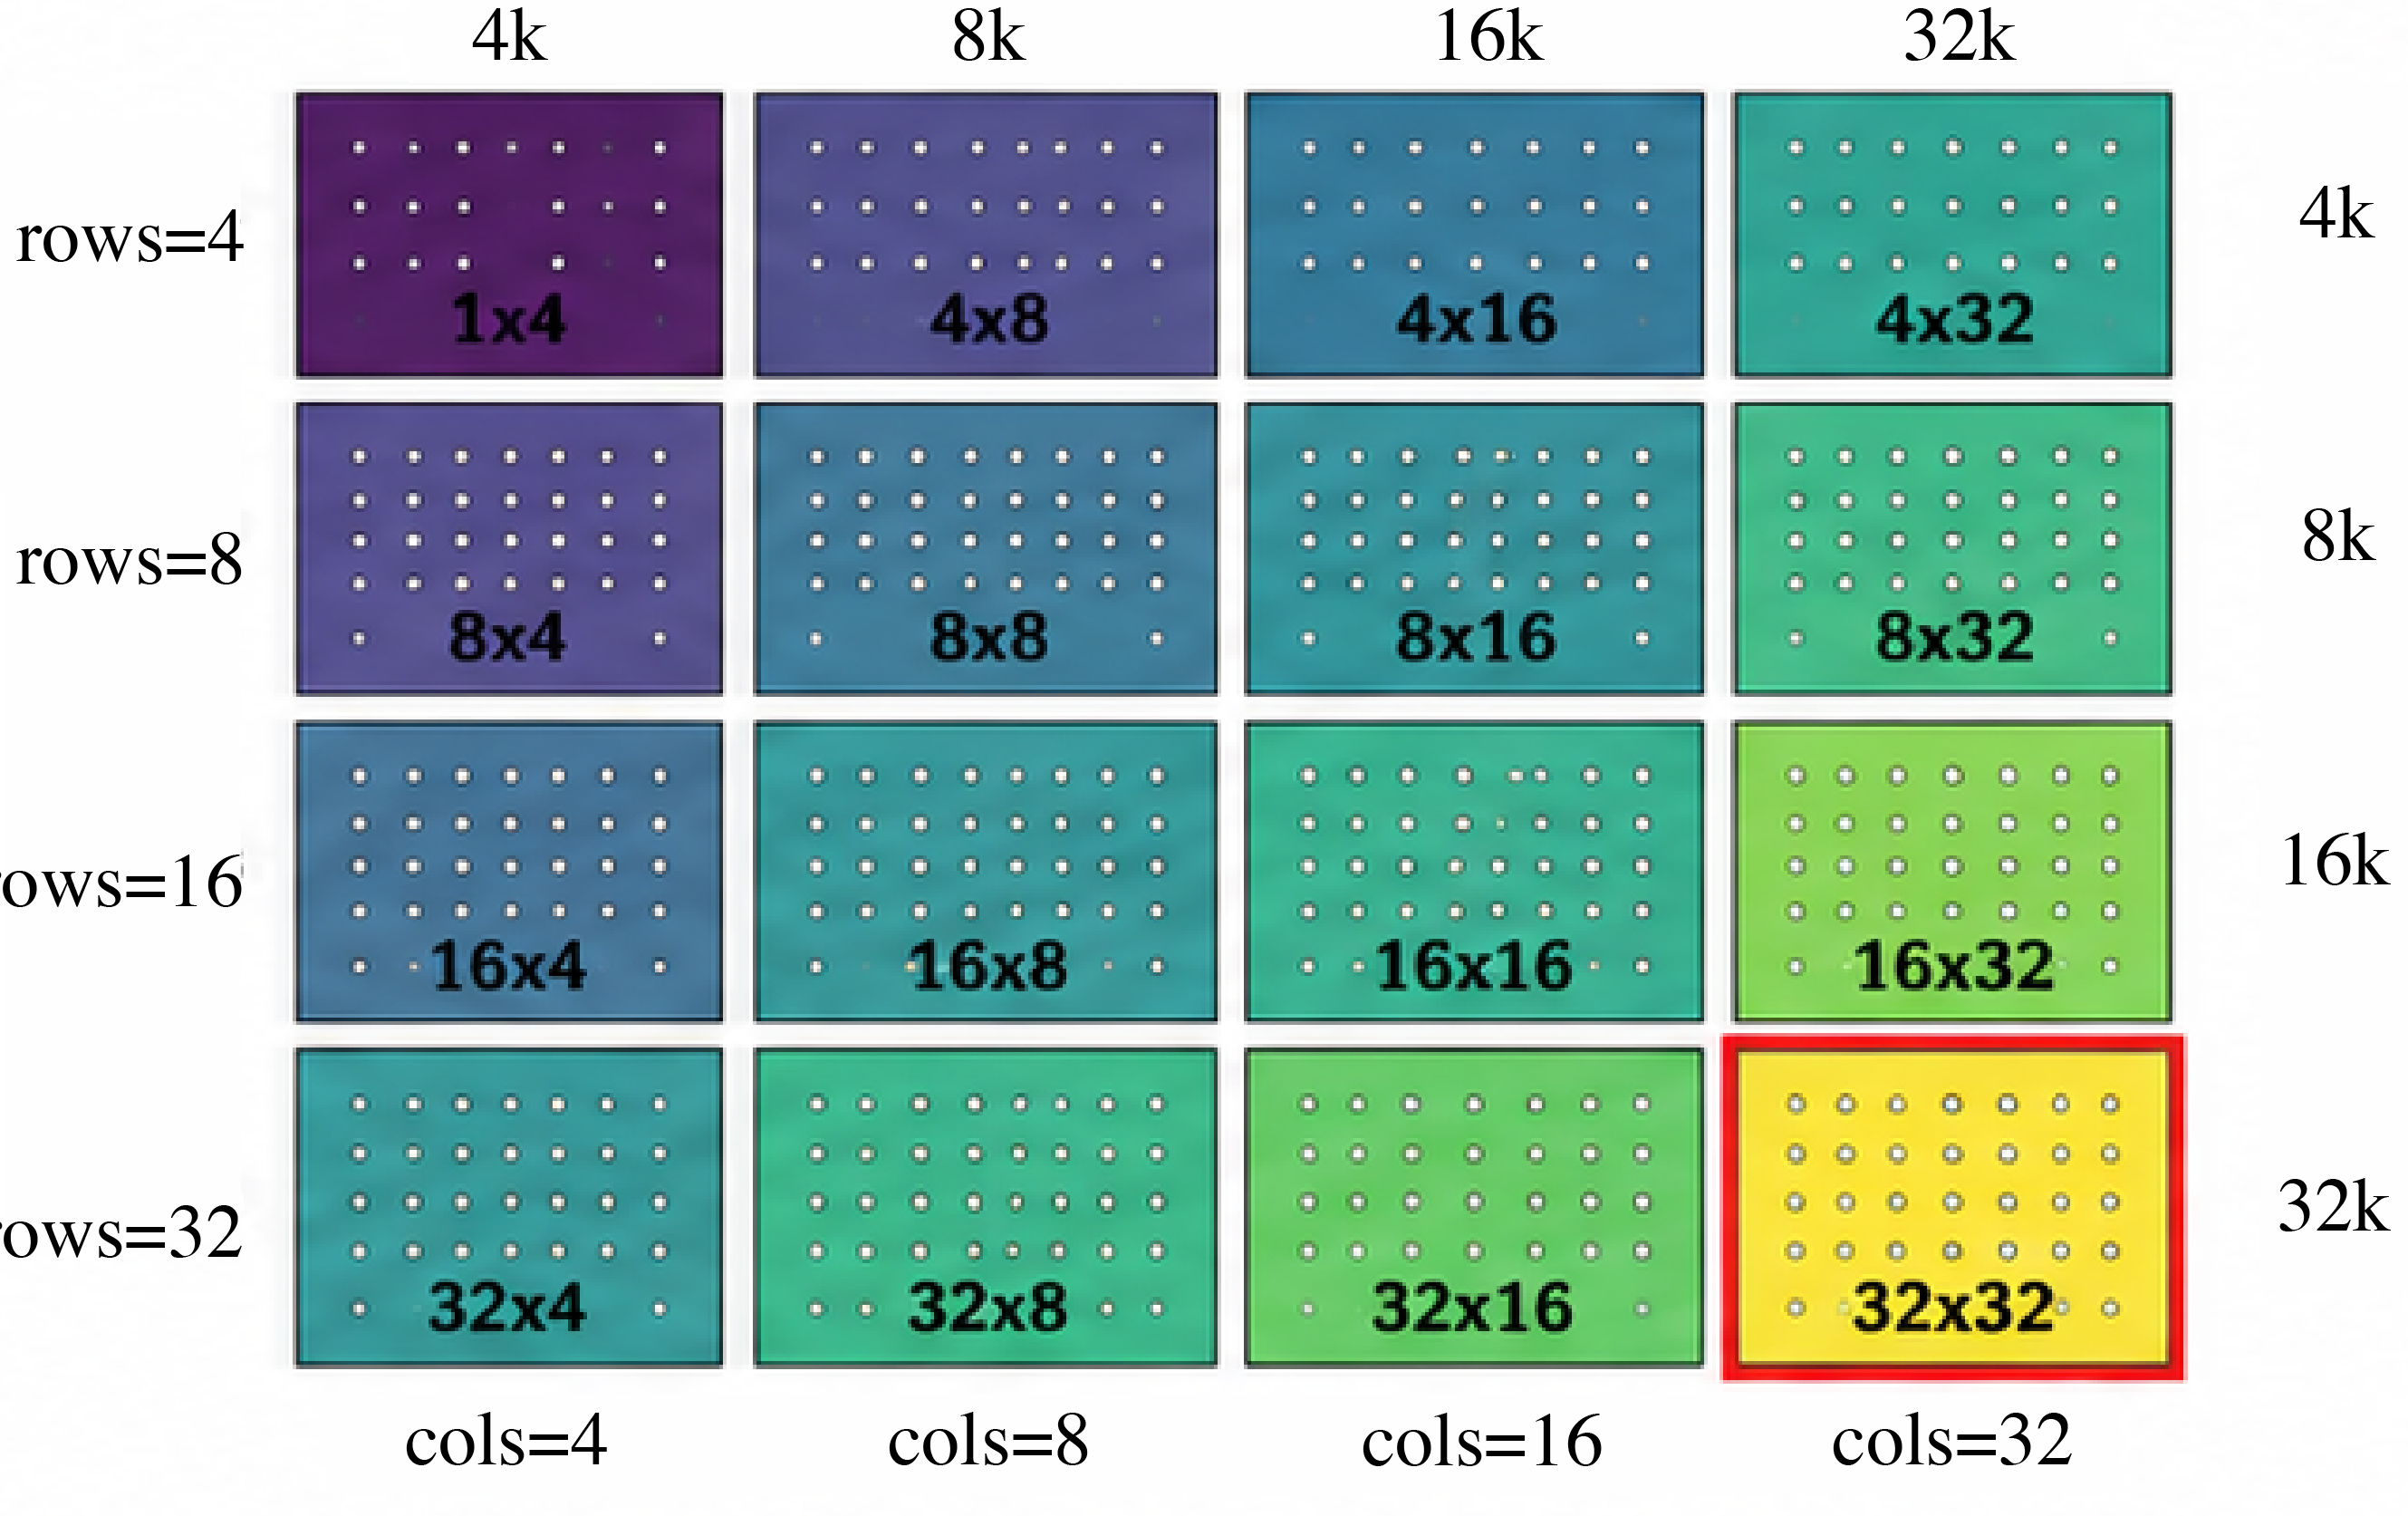
\includegraphics[width=0.48\textwidth]{figs4/tiles.png}
\caption{
Example per-layer tiling cache for EfficientNet-B7 layer L4.
Left: Timeloop-evaluated candidates plotted by fused/on-chip cost
\(T_{\min}(c)\) and spilled/off-chip cost \(T_{\max}(c)\); the frontier shows
non-dominated choices and the star is the LP-rounded selection. Right: the
16 tiling choices; labels such as \(4\times4\),
\(8\times8\), and \(32\times32\) denote active tile rows/columns inside the
fixed accelerator, white dots indicate active PE/MAC sites.
These are schedule choices, not different chips.
}
\label{fig:tiles}
\end{figure}

\begin{figure}[ht!]
    \centering
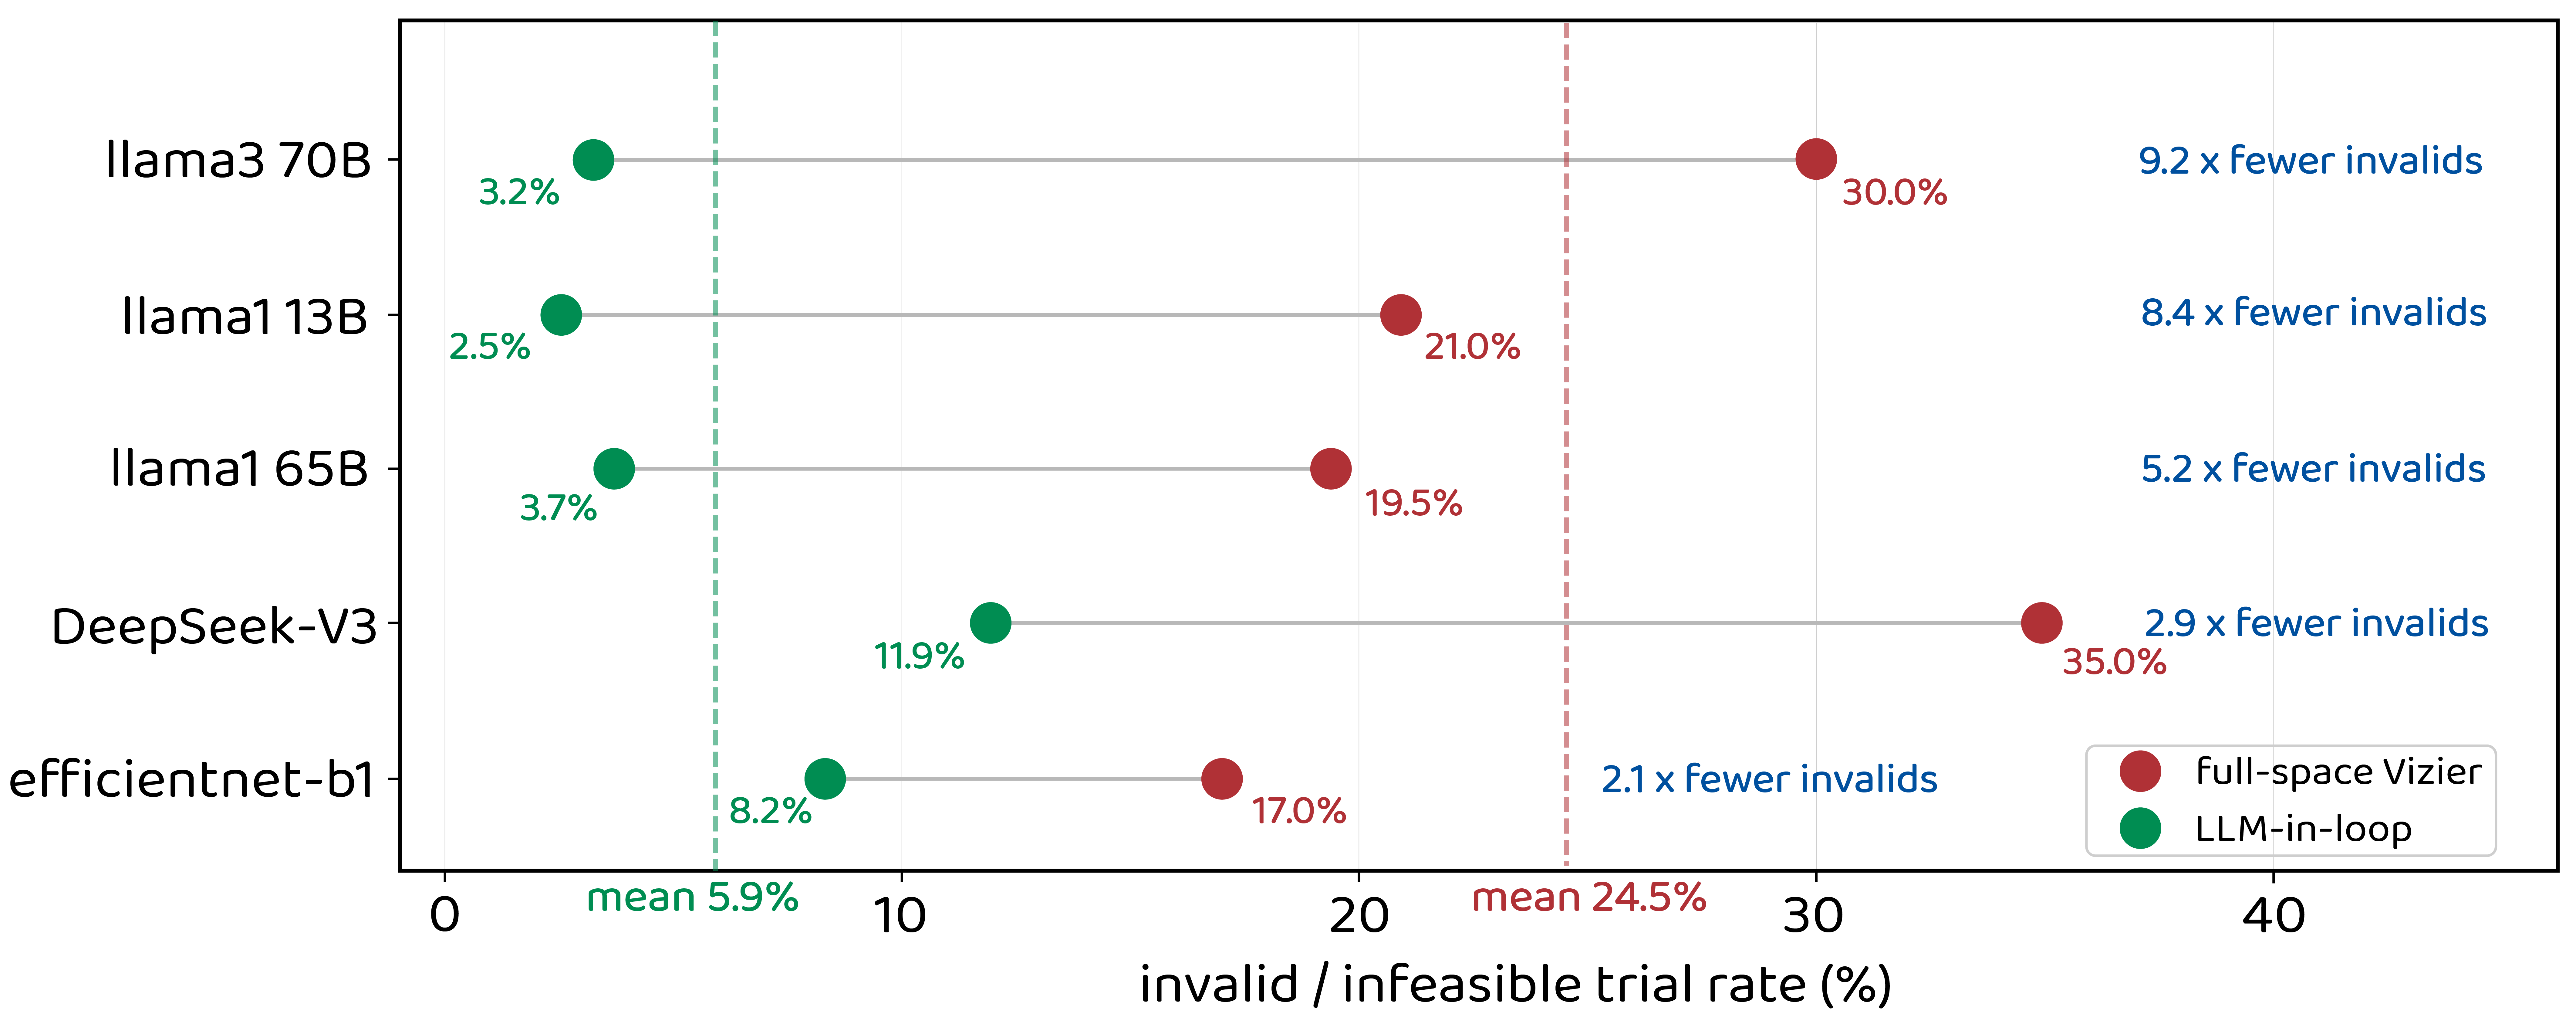
\includegraphics[width=0.85\linewidth]{fig3/llm_guide_v1.png}
\caption{Invalid/infeasible trial rate (\%) for full-space Vizier vs.\ LLM-in-loop across five workloads. The LLM Architect reduces the mean invalid rate from 24.5\% to 5.9\% (4.1$\times$ reduction), with the largest gains on LLM workloads where the hardware search space is most prone to infeasible configurations.}\label{fig:llm}
\end{figure}
